% Generated by Sphinx.
\def\sphinxdocclass{report}
\documentclass[letterpaper,10pt,english]{sphinxmanual}
\usepackage[utf8]{inputenc}
\DeclareUnicodeCharacter{00A0}{\nobreakspace}
\usepackage[T1]{fontenc}
\usepackage{babel}
\usepackage{times}
\usepackage[Bjarne]{fncychap}
\usepackage{longtable}
\usepackage{sphinx}
\usepackage{multirow}


\title{ViCE Documentation}
\date{May 19, 2012}
\release{0.0.1}
\author{Edwin Marshall}
\newcommand{\sphinxlogo}{}
\renewcommand{\releasename}{Release}
\makeindex

\makeatletter
\def\PYG@reset{\let\PYG@it=\relax \let\PYG@bf=\relax%
    \let\PYG@ul=\relax \let\PYG@tc=\relax%
    \let\PYG@bc=\relax \let\PYG@ff=\relax}
\def\PYG@tok#1{\csname PYG@tok@#1\endcsname}
\def\PYG@toks#1+{\ifx\relax#1\empty\else%
    \PYG@tok{#1}\expandafter\PYG@toks\fi}
\def\PYG@do#1{\PYG@bc{\PYG@tc{\PYG@ul{%
    \PYG@it{\PYG@bf{\PYG@ff{#1}}}}}}}
\def\PYG#1#2{\PYG@reset\PYG@toks#1+\relax+\PYG@do{#2}}

\expandafter\def\csname PYG@tok@gd\endcsname{\def\PYG@tc##1{\textcolor[rgb]{0.63,0.00,0.00}{##1}}}
\expandafter\def\csname PYG@tok@gu\endcsname{\let\PYG@bf=\textbf\def\PYG@tc##1{\textcolor[rgb]{0.50,0.00,0.50}{##1}}}
\expandafter\def\csname PYG@tok@gt\endcsname{\def\PYG@tc##1{\textcolor[rgb]{0.00,0.25,0.82}{##1}}}
\expandafter\def\csname PYG@tok@gs\endcsname{\let\PYG@bf=\textbf}
\expandafter\def\csname PYG@tok@gr\endcsname{\def\PYG@tc##1{\textcolor[rgb]{1.00,0.00,0.00}{##1}}}
\expandafter\def\csname PYG@tok@cm\endcsname{\let\PYG@it=\textit\def\PYG@tc##1{\textcolor[rgb]{0.25,0.50,0.56}{##1}}}
\expandafter\def\csname PYG@tok@vg\endcsname{\def\PYG@tc##1{\textcolor[rgb]{0.73,0.38,0.84}{##1}}}
\expandafter\def\csname PYG@tok@m\endcsname{\def\PYG@tc##1{\textcolor[rgb]{0.13,0.50,0.31}{##1}}}
\expandafter\def\csname PYG@tok@mh\endcsname{\def\PYG@tc##1{\textcolor[rgb]{0.13,0.50,0.31}{##1}}}
\expandafter\def\csname PYG@tok@cs\endcsname{\def\PYG@tc##1{\textcolor[rgb]{0.25,0.50,0.56}{##1}}\def\PYG@bc##1{\setlength{\fboxsep}{0pt}\colorbox[rgb]{1.00,0.94,0.94}{\strut ##1}}}
\expandafter\def\csname PYG@tok@ge\endcsname{\let\PYG@it=\textit}
\expandafter\def\csname PYG@tok@vc\endcsname{\def\PYG@tc##1{\textcolor[rgb]{0.73,0.38,0.84}{##1}}}
\expandafter\def\csname PYG@tok@il\endcsname{\def\PYG@tc##1{\textcolor[rgb]{0.13,0.50,0.31}{##1}}}
\expandafter\def\csname PYG@tok@go\endcsname{\def\PYG@tc##1{\textcolor[rgb]{0.19,0.19,0.19}{##1}}}
\expandafter\def\csname PYG@tok@cp\endcsname{\def\PYG@tc##1{\textcolor[rgb]{0.00,0.44,0.13}{##1}}}
\expandafter\def\csname PYG@tok@gi\endcsname{\def\PYG@tc##1{\textcolor[rgb]{0.00,0.63,0.00}{##1}}}
\expandafter\def\csname PYG@tok@gh\endcsname{\let\PYG@bf=\textbf\def\PYG@tc##1{\textcolor[rgb]{0.00,0.00,0.50}{##1}}}
\expandafter\def\csname PYG@tok@ni\endcsname{\let\PYG@bf=\textbf\def\PYG@tc##1{\textcolor[rgb]{0.84,0.33,0.22}{##1}}}
\expandafter\def\csname PYG@tok@nl\endcsname{\let\PYG@bf=\textbf\def\PYG@tc##1{\textcolor[rgb]{0.00,0.13,0.44}{##1}}}
\expandafter\def\csname PYG@tok@nn\endcsname{\let\PYG@bf=\textbf\def\PYG@tc##1{\textcolor[rgb]{0.05,0.52,0.71}{##1}}}
\expandafter\def\csname PYG@tok@no\endcsname{\def\PYG@tc##1{\textcolor[rgb]{0.38,0.68,0.84}{##1}}}
\expandafter\def\csname PYG@tok@na\endcsname{\def\PYG@tc##1{\textcolor[rgb]{0.25,0.44,0.63}{##1}}}
\expandafter\def\csname PYG@tok@nb\endcsname{\def\PYG@tc##1{\textcolor[rgb]{0.00,0.44,0.13}{##1}}}
\expandafter\def\csname PYG@tok@nc\endcsname{\let\PYG@bf=\textbf\def\PYG@tc##1{\textcolor[rgb]{0.05,0.52,0.71}{##1}}}
\expandafter\def\csname PYG@tok@nd\endcsname{\let\PYG@bf=\textbf\def\PYG@tc##1{\textcolor[rgb]{0.33,0.33,0.33}{##1}}}
\expandafter\def\csname PYG@tok@ne\endcsname{\def\PYG@tc##1{\textcolor[rgb]{0.00,0.44,0.13}{##1}}}
\expandafter\def\csname PYG@tok@nf\endcsname{\def\PYG@tc##1{\textcolor[rgb]{0.02,0.16,0.49}{##1}}}
\expandafter\def\csname PYG@tok@si\endcsname{\let\PYG@it=\textit\def\PYG@tc##1{\textcolor[rgb]{0.44,0.63,0.82}{##1}}}
\expandafter\def\csname PYG@tok@s2\endcsname{\def\PYG@tc##1{\textcolor[rgb]{0.25,0.44,0.63}{##1}}}
\expandafter\def\csname PYG@tok@vi\endcsname{\def\PYG@tc##1{\textcolor[rgb]{0.73,0.38,0.84}{##1}}}
\expandafter\def\csname PYG@tok@nt\endcsname{\let\PYG@bf=\textbf\def\PYG@tc##1{\textcolor[rgb]{0.02,0.16,0.45}{##1}}}
\expandafter\def\csname PYG@tok@nv\endcsname{\def\PYG@tc##1{\textcolor[rgb]{0.73,0.38,0.84}{##1}}}
\expandafter\def\csname PYG@tok@s1\endcsname{\def\PYG@tc##1{\textcolor[rgb]{0.25,0.44,0.63}{##1}}}
\expandafter\def\csname PYG@tok@gp\endcsname{\let\PYG@bf=\textbf\def\PYG@tc##1{\textcolor[rgb]{0.78,0.36,0.04}{##1}}}
\expandafter\def\csname PYG@tok@sh\endcsname{\def\PYG@tc##1{\textcolor[rgb]{0.25,0.44,0.63}{##1}}}
\expandafter\def\csname PYG@tok@ow\endcsname{\let\PYG@bf=\textbf\def\PYG@tc##1{\textcolor[rgb]{0.00,0.44,0.13}{##1}}}
\expandafter\def\csname PYG@tok@sx\endcsname{\def\PYG@tc##1{\textcolor[rgb]{0.78,0.36,0.04}{##1}}}
\expandafter\def\csname PYG@tok@bp\endcsname{\def\PYG@tc##1{\textcolor[rgb]{0.00,0.44,0.13}{##1}}}
\expandafter\def\csname PYG@tok@c1\endcsname{\let\PYG@it=\textit\def\PYG@tc##1{\textcolor[rgb]{0.25,0.50,0.56}{##1}}}
\expandafter\def\csname PYG@tok@kc\endcsname{\let\PYG@bf=\textbf\def\PYG@tc##1{\textcolor[rgb]{0.00,0.44,0.13}{##1}}}
\expandafter\def\csname PYG@tok@c\endcsname{\let\PYG@it=\textit\def\PYG@tc##1{\textcolor[rgb]{0.25,0.50,0.56}{##1}}}
\expandafter\def\csname PYG@tok@mf\endcsname{\def\PYG@tc##1{\textcolor[rgb]{0.13,0.50,0.31}{##1}}}
\expandafter\def\csname PYG@tok@err\endcsname{\def\PYG@bc##1{\setlength{\fboxsep}{0pt}\fcolorbox[rgb]{1.00,0.00,0.00}{1,1,1}{\strut ##1}}}
\expandafter\def\csname PYG@tok@kd\endcsname{\let\PYG@bf=\textbf\def\PYG@tc##1{\textcolor[rgb]{0.00,0.44,0.13}{##1}}}
\expandafter\def\csname PYG@tok@ss\endcsname{\def\PYG@tc##1{\textcolor[rgb]{0.32,0.47,0.09}{##1}}}
\expandafter\def\csname PYG@tok@sr\endcsname{\def\PYG@tc##1{\textcolor[rgb]{0.14,0.33,0.53}{##1}}}
\expandafter\def\csname PYG@tok@mo\endcsname{\def\PYG@tc##1{\textcolor[rgb]{0.13,0.50,0.31}{##1}}}
\expandafter\def\csname PYG@tok@mi\endcsname{\def\PYG@tc##1{\textcolor[rgb]{0.13,0.50,0.31}{##1}}}
\expandafter\def\csname PYG@tok@kn\endcsname{\let\PYG@bf=\textbf\def\PYG@tc##1{\textcolor[rgb]{0.00,0.44,0.13}{##1}}}
\expandafter\def\csname PYG@tok@o\endcsname{\def\PYG@tc##1{\textcolor[rgb]{0.40,0.40,0.40}{##1}}}
\expandafter\def\csname PYG@tok@kr\endcsname{\let\PYG@bf=\textbf\def\PYG@tc##1{\textcolor[rgb]{0.00,0.44,0.13}{##1}}}
\expandafter\def\csname PYG@tok@s\endcsname{\def\PYG@tc##1{\textcolor[rgb]{0.25,0.44,0.63}{##1}}}
\expandafter\def\csname PYG@tok@kp\endcsname{\def\PYG@tc##1{\textcolor[rgb]{0.00,0.44,0.13}{##1}}}
\expandafter\def\csname PYG@tok@w\endcsname{\def\PYG@tc##1{\textcolor[rgb]{0.73,0.73,0.73}{##1}}}
\expandafter\def\csname PYG@tok@kt\endcsname{\def\PYG@tc##1{\textcolor[rgb]{0.56,0.13,0.00}{##1}}}
\expandafter\def\csname PYG@tok@sc\endcsname{\def\PYG@tc##1{\textcolor[rgb]{0.25,0.44,0.63}{##1}}}
\expandafter\def\csname PYG@tok@sb\endcsname{\def\PYG@tc##1{\textcolor[rgb]{0.25,0.44,0.63}{##1}}}
\expandafter\def\csname PYG@tok@k\endcsname{\let\PYG@bf=\textbf\def\PYG@tc##1{\textcolor[rgb]{0.00,0.44,0.13}{##1}}}
\expandafter\def\csname PYG@tok@se\endcsname{\let\PYG@bf=\textbf\def\PYG@tc##1{\textcolor[rgb]{0.25,0.44,0.63}{##1}}}
\expandafter\def\csname PYG@tok@sd\endcsname{\let\PYG@it=\textit\def\PYG@tc##1{\textcolor[rgb]{0.25,0.44,0.63}{##1}}}

\def\PYGZbs{\char`\\}
\def\PYGZus{\char`\_}
\def\PYGZob{\char`\{}
\def\PYGZcb{\char`\}}
\def\PYGZca{\char`\^}
\def\PYGZam{\char`\&}
\def\PYGZlt{\char`\<}
\def\PYGZgt{\char`\>}
\def\PYGZsh{\char`\#}
\def\PYGZpc{\char`\%}
\def\PYGZdl{\char`\$}
\def\PYGZti{\char`\~}
% for compatibility with earlier versions
\def\PYGZat{@}
\def\PYGZlb{[}
\def\PYGZrb{]}
\makeatother

\begin{document}

\maketitle
\tableofcontents
\phantomsection\label{index::doc}


\textsc{ViCE} (Virtual Card-game Engine) is an open source, portable, modular
framework for playing and creating \textsc{TCGs} (Trading Card Games). This
manual outlines ViCE's design principles, describes its various features from
three perspectives (which we refer to as roles), and even includes reference
documentation for the public API.

\begin{notice}{note}{Note:}
While there are subtle differences between the Trading Card Games and
Collectible Card Games, in the interest of simplicity, this manual refers
to them collectively (no pun intended) as TCGs.
\end{notice}


\part{How This Manual is Organized}
\label{index:introduction}\label{index:how-this-manual-is-organized}
This book is organized into four parts, the first three of which being guides
modeled after their respective roles:


\chapter{Player Guide}
\label{player_guide/player_index:player-guide}\label{player_guide/player_index::doc}
Welcome to ViCe's official player guide. It describes ViCE's UI so that you
can quickly get started playing your favorite TCGs on ViCE, find other
players, and even run your own ViCE server so that you can host tournaments
or keep track of stats.


\chapter{Designer Guide}
\label{designer_guide/designer_index:designer-guide}\label{designer_guide/designer_index::doc}
Welcome to ViCe's official designer guide. It describes ViCE's high-level
components so that you can port your favorite TCG's to ViCE, improve
the quality of existing ports, or create a new TCG from scratch.


\chapter{Developer Guide}
\label{developer_guide/developer_index::doc}\label{developer_guide/developer_index:developer-guide}
This guide discusses the underlying patterns and idioms used when developing
ViCE.


\section{Architecture}
\label{developer_guide/architecture::doc}\label{developer_guide/architecture:architecture}
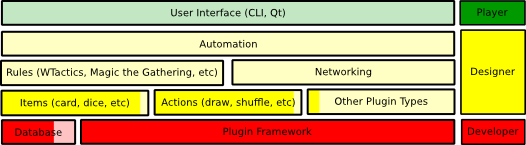
\includegraphics{stack_diagram.png}

As you can see from the architecture stack diagram above, ViCE's core is
composed of the plugin framework and database layer \footnote{
Custom data types such as the PropertyDict are also part of ViCE's
core, but they were left out of the chart for the sake of simplicity.
}. Item, Action, and other,
yet to be developed plugin types sit directly on these components. While not
yet started, other features and abstractions suitable for designers and
players will then be built on top of these.

\begin{notice}{note}{Note:}
The opacity of each box represents an approximation of how complete the
represented component is.
\end{notice}


\subsection{Plugin Framework}
\label{developer_guide/architecture:plugin-framework}
ViCE's plugin framework is based on the simple fact that all new-style
classes \footnote{
\href{http://www.python.org/doc/newstyle/}{http://www.python.org/doc/newstyle/}
} in python know about their subclasses. All plugins \footnote{
Only plugins which are meant to be instantiated need assign the NAME
class attribute. That is, plugin base classes should \emph{not} assign
this attribute.
} must
be given a name by assigning the class attribute NAME. It is through this
name that plugins are identified, and without it, a plugin won't be
discoverable.

For information on the different plugin types and their roles, please
refer to the {\hyperref[designer_guide/designer_index::doc]{\emph{Designer Guide}}}.


\subsection{Database Layer}
\label{developer_guide/architecture:database-layer}
\begin{notice}{note}{Note:}
Not all of SQLAlchemy's API has been abstracted, so some things are
not yet possible. For more information, consult the {\hyperref[api_reference::doc]{\emph{API Reference}}}.
\end{notice}

The database layer is an abstraction on top of
the already excellent abstraction layer \href{http://sqlalchemy.org}{SQLAlchemy}.
While this might seem excessive, it is necessary for three reasons:
\begin{enumerate}
\item {} 
Flexibility: Tucking the implementation details behind a simple API allows
us to not only change the underlying module used if we ever decide to, but
also selectively reimplement features that we feel aren't covered well by
the underlying module.

\item {} 
Brevity: ViCE's database API is much more concise than SQLAlchemy alone,
serves to simplify code, as well as the learning of the API itself.

\item {} 
Seamless Integration: Since the database layer sits next to the plugin
framework and beneath all other components, it's tightly integrated \footnote{
Note that we did not say ``tightly coupled''. As such, it is possible
for alternate implementations to be used.
}
with the rest of the framework.

\end{enumerate}

Currently, the database layer is not implemented as a plugin because
SQLAlchemy provides a unified API on top of many
\textsc{RDBMSs} (Relational Database Management Systems).


\strong{See Also:}

\begin{itemize}
\item {} 
{\hyperref[api_reference:vice]{\emph{vice -- Main package, also provides PropertyDict}}}

\item {} 
{\hyperref[api_reference:vice-database]{\emph{vice.database -- Database abstraction and integration}}}

\item {} 
{\hyperref[api_reference:vice-plugins]{\emph{vice.plugins -- Infrastructure for implementing plugins}}}

\end{itemize}




\chapter{API Reference}
\label{api_reference:api-reference}\label{api_reference::doc}

\section{vice -- Main package, also provides PropertyDict}
\label{api_reference:vice-main-package-also-provides-propertydict}\label{api_reference:vice}\index{PropertyDict (class in vice)}

\begin{fulllineitems}
\phantomsection\label{api_reference:vice.PropertyDict}\pysigline{\strong{class }\code{vice.}\bfcode{PropertyDict}}
A dict subclass that allows values to be retrieved by accessing their
keys as properties.

PropertyDict provides a dictionary whose key:value pairs may be
assigned in the conventional brace notation (foo{[}'bar'{]} = `baz'),
or in the more elegant object:property notation (foo.bar = `baz').
Beyond this subtle addition, they behave identically to regular
dictionaries.

\end{fulllineitems}



\section{vice.database -- Database abstraction and integration}
\label{api_reference:vice-database-database-abstraction-and-integration}\label{api_reference:module-vice.database}\label{api_reference:vice-database}\index{vice.database (module)}\index{Database (class in vice.database)}

\begin{fulllineitems}
\phantomsection\label{api_reference:vice.database.Database}\pysiglinewithargsret{\strong{class }\code{vice.database.}\bfcode{Database}}{\emph{URI=None}, \emph{echo=False}}{}
Abstraction layer on top of SQLAlchemy's interface.

While SQLAlchemy abstracts the particulars of different
database backends and the subtle ways SQL may differ within them,
this Database class abstracts the SQLAlchemy API into something more
simple, meanwhile adding facilities that make it integrate better with
ViCE's plugin architecture.
\index{connect() (vice.database.Database method)}

\begin{fulllineitems}
\phantomsection\label{api_reference:vice.database.Database.connect}\pysiglinewithargsret{\bfcode{connect}}{\emph{URI}, \emph{echo=False}}{}
Connects to an existing database, or creates a new one if one
isn't found.

URI may be any URI recognized by SQLAlchemy, and generally follows
the form:

\begin{Verbatim}[commandchars=\\\{\}]
\PYG{l+s}{"}\PYG{l+s}{\PYGZlt{}protocol\PYGZgt{}:///\PYGZlt{}location\PYGZgt{}}\PYG{l+s}{"}
\end{Verbatim}

For example:

\begin{Verbatim}[commandchars=\\\{\}]
\PYG{l+s}{"}\PYG{l+s}{sqlite:///wtactics.db}\PYG{l+s}{"}
\end{Verbatim}

echo determines whether or not SQL statements are echoed to stdout
after each operation.

\end{fulllineitems}

\index{create\_record() (vice.database.Database method)}

\begin{fulllineitems}
\phantomsection\label{api_reference:vice.database.Database.create_record}\pysiglinewithargsret{\bfcode{create\_record}}{\emph{table\_name}, \emph{**parameters}}{}
Creates a record in table\_name, using parameters.

Example:

\begin{Verbatim}[commandchars=\\\{\}]
\PYG{n}{db}\PYG{o}{.}\PYG{n}{create\PYGZus{}record}\PYG{p}{(}\PYG{l+s}{'}\PYG{l+s}{cards}\PYG{l+s}{'}\PYG{p}{,}
    \PYG{c}{\PYGZsh{} note that id is auto-incremented, so isn't specified}
    \PYG{n}{name} \PYG{o}{=} \PYG{l+s}{'}\PYG{l+s}{Imp}\PYG{l+s}{'}\PYG{p}{,}
    \PYG{n}{atk} \PYG{o}{=} \PYG{l+m+mi}{2}\PYG{p}{,}
    \PYG{n}{def\PYGZus{}} \PYG{o}{=} \PYG{l+m+mi}{2}
\PYG{p}{)}
\end{Verbatim}

\end{fulllineitems}

\index{create\_table() (vice.database.Database method)}

\begin{fulllineitems}
\phantomsection\label{api_reference:vice.database.Database.create_table}\pysiglinewithargsret{\bfcode{create\_table}}{\emph{table\_name}, \emph{**column\_attrs}}{}
Creates a table in the database named table\_name, with columns
whose attributes match column\_attrs.

table\_name may be anything you wish, but if it so happens to be a
reserved word in Python (eg. `def'), then you must suffix it with
an underscore (`\_'). You needn't worry, however, since the
trailing underscore is removed inside the actual database.

All remaining keyword arguments will be processed as column
attributes where the keys should be valid column names, and the values
should be arguments to column types.
\begin{description}
\item[{Valid column types are currently:}] \leavevmode\begin{itemize}
\item {} 
string() -- Represents an string column.

\item {} 
integer() -- Represents an integer column .

\end{itemize}

\end{description}

Arguments may be passed to these column types to further specify
restrictions on data or relationships.
\begin{description}
\item[{Valid arguments are currently:}] \leavevmode
primary\_key=True -- Marks the column as the primary key.

\end{description}

Example:

\begin{Verbatim}[commandchars=\\\{\}]
\PYG{n}{db}\PYG{o}{.}\PYG{n}{create\PYGZus{}table}\PYG{p}{(}\PYG{l+s}{'}\PYG{l+s}{cards}\PYG{l+s}{'}\PYG{p}{,}
    \PYG{n+nb}{id} \PYG{o}{=} \PYG{n}{integer}\PYG{p}{(}\PYG{n}{primary\PYGZus{}key}\PYG{o}{=}\PYG{n+nb+bp}{True}\PYG{p}{)}\PYG{p}{,}
    \PYG{n}{name} \PYG{o}{=} \PYG{n}{string}\PYG{p}{(}\PYG{p}{)}\PYG{p}{,}
    \PYG{n}{atk} \PYG{o}{=} \PYG{n}{integer}\PYG{p}{(}\PYG{p}{)}\PYG{p}{,}
    \PYG{n}{def\PYGZus{}} \PYG{o}{=} \PYG{n}{integer}\PYG{p}{(}\PYG{p}{)} \PYG{c}{\PYGZsh{} notice the trailing underscore}
\PYG{p}{)}
\end{Verbatim}

\begin{notice}{note}{Note:}
Since column\_attrs is a dictionary, definition order is
arbitrary, and thus the order in which the columns is
specified may differ from what you expect when examining the
resulting database.
\end{notice}

\end{fulllineitems}

\index{select() (vice.database.Database method)}

\begin{fulllineitems}
\phantomsection\label{api_reference:vice.database.Database.select}\pysiglinewithargsret{\bfcode{select}}{\emph{tables}, \emph{**kwargs}}{}
Selects all records of the given tables.

tables is a list of table names.

\begin{notice}{warning}{Warning:}
The interface is mostly ported directly from SQLAlchemy. In
the future, a simpler interface will be implemented, most
probably named ``find'', and this one will be deprecated for
immediate removal.
\end{notice}

\end{fulllineitems}

\index{tables (vice.database.Database attribute)}

\begin{fulllineitems}
\phantomsection\label{api_reference:vice.database.Database.tables}\pysigline{\bfcode{tables}}
Returns a list of table names for the current database object.

\end{fulllineitems}


\end{fulllineitems}

\index{integer() (in module vice.database)}

\begin{fulllineitems}
\phantomsection\label{api_reference:vice.database.integer}\pysiglinewithargsret{\code{vice.database.}\bfcode{integer}}{\emph{**kwargs}}{}
Returns a kwargs dictionary suitable for creating an SQLAlchemy
Integer column.

\end{fulllineitems}

\index{string() (in module vice.database)}

\begin{fulllineitems}
\phantomsection\label{api_reference:vice.database.string}\pysiglinewithargsret{\code{vice.database.}\bfcode{string}}{\emph{**kwargs}}{}
Returns a kwargs dictionary suitable for creating an SQLAlchemy
String column.

\end{fulllineitems}



\section{vice.plugins -- Infrastructure for implementing plugins}
\label{api_reference:vice-plugins}\label{api_reference:module-vice.plugins}\label{api_reference:vice-plugins-infrastructure-for-implementing-plugins}\index{vice.plugins (module)}\index{Plugin (class in vice.plugins)}

\begin{fulllineitems}
\phantomsection\label{api_reference:vice.plugins.Plugin}\pysigline{\strong{class }\code{vice.plugins.}\bfcode{Plugin}}
Base class for all new plugin types.

All new plugin types are created by subclassing Plugin. In
most cases, you will want to inherit from a Plugin subclass
rather than directly from Plugin itself.

All new plugins must have a NAME class attribute, which is used mainly
for plugin discovery.
\index{plugins() (vice.plugins.Plugin class method)}

\begin{fulllineitems}
\phantomsection\label{api_reference:vice.plugins.Plugin.plugins}\pysiglinewithargsret{\strong{classmethod }\bfcode{plugins}}{}{}
Returns a plugin's subclasses as a vice.PropertyDict.

This PropertyDict's keys are plugin names and values are the plugin
classes that correspond with those names. A common idiom is to
assign the return value to a variable to ease the access to
available plugins:

\begin{Verbatim}[commandchars=\\\{\}]
\PYG{n}{foo\PYGZus{}plugins} \PYG{o}{=} \PYG{n}{Foo}\PYG{o}{.}\PYG{n}{plugins}\PYG{p}{(}\PYG{p}{)}
\PYG{n}{baz} \PYG{o}{=} \PYG{n}{foo\PYGZus{}plugins}\PYG{o}{.}\PYG{n}{Baz}\PYG{p}{(}\PYG{n}{x}\PYG{p}{,} \PYG{n}{y}\PYG{p}{)}
\end{Verbatim}

\end{fulllineitems}


\end{fulllineitems}



\subsection{vice.plugins.actions -- Built-in action plugins}
\label{api_reference:module-vice.plugins.actions}\label{api_reference:vice-plugins-actions-built-in-action-plugins}\label{api_reference:vice-plugins-actions}\index{vice.plugins.actions (module)}\index{Action (class in vice.plugins.actions)}

\begin{fulllineitems}
\phantomsection\label{api_reference:vice.plugins.actions.Action}\pysigline{\strong{class }\code{vice.plugins.actions.}\bfcode{Action}}
Callable plugin that provides general operations for Item plugins.

An action is a class which acts like a generic function that operates
on Item plugins. This approach is more flexible, extensible, and less
repetitious than implementing methods directly within a subclass.

To create a new action, define an Action subclass, override NAME (by
convention, lowercase for actions), and finally override \_\_call\_\_:

\begin{Verbatim}[commandchars=\\\{\}]
\PYG{k}{class} \PYG{n+nc}{Foo}\PYG{p}{(}\PYG{n}{Action}\PYG{p}{)}\PYG{p}{:}
    \PYG{n}{NAME} \PYG{o}{=} \PYG{l+s}{'}\PYG{l+s}{foo}\PYG{l+s}{'}

    \PYG{k}{def} \PYG{n+nf}{\PYGZus{}\PYGZus{}call\PYGZus{}\PYGZus{}}\PYG{p}{(}\PYG{n}{cls}\PYG{p}{)}\PYG{p}{:}
        \PYG{k}{return} \PYG{l+s}{'}\PYG{l+s}{bar}\PYG{l+s}{'}
\end{Verbatim}

Alternatively, you may define a simple function and pass that to
Action.new:

\begin{Verbatim}[commandchars=\\\{\}]
\PYG{k}{def} \PYG{n+nf}{foo}\PYG{p}{(}\PYG{n}{cls}\PYG{p}{)}\PYG{p}{:}
    \PYG{k}{return} \PYG{l+s}{'}\PYG{l+s}{bar}\PYG{l+s}{'}

\PYG{n}{Action}\PYG{o}{.}\PYG{n}{new}\PYG{p}{(}\PYG{n}{foo}\PYG{p}{)}
\end{Verbatim}
\index{new() (vice.plugins.actions.Action class method)}

\begin{fulllineitems}
\phantomsection\label{api_reference:vice.plugins.actions.Action.new}\pysiglinewithargsret{\strong{classmethod }\bfcode{new}}{\emph{function}}{}
Convenience method used to help simply creation of new actions.

The function's name is converted to title case and used as the name
of the class, and it's original form is used as the Plugin's NAME.

When defining the function, make sure the first argument is cls,
since this will be used as the class's \_\_call\_\_ special method

\end{fulllineitems}

\index{plugins() (vice.plugins.actions.Action class method)}

\begin{fulllineitems}
\phantomsection\label{api_reference:vice.plugins.actions.Action.plugins}\pysiglinewithargsret{\strong{classmethod }\bfcode{plugins}}{\emph{*args}, \emph{**kwargs}}{}
Acts similarly to Plugin.plugins(), except that it returns
instances of the plugin classes, rather than the classes
themselves.

\end{fulllineitems}


\end{fulllineitems}



\subsection{vice.plugins.items -- Built-in item plugins}
\label{api_reference:vice-plugins-items-built-in-item-plugins}\label{api_reference:module-vice.plugins.items}\label{api_reference:vice-plugins-items}\index{vice.plugins.items (module)}\index{Item (class in vice.plugins.items)}

\begin{fulllineitems}
\phantomsection\label{api_reference:vice.plugins.items.Item}\pysigline{\strong{class }\code{vice.plugins.items.}\bfcode{Item}}
Plugin that represents a games tangible objects.

An item is any object within a card game that can be interacted
with. The most obvious example of this would be the game's cards,
but things such as tokens and dice would be implemented as items
as well.

To create a new item, define a new Item subclass, override the NAME
attribute (by convention, uppercase for items), and finally override
ATTRIBUTES with a sequence of strings:

\begin{Verbatim}[commandchars=\\\{\}]
\PYG{k}{class} \PYG{n+nc}{Card}\PYG{p}{(}\PYG{n}{Item}\PYG{p}{)}\PYG{p}{:}
    \PYG{n}{NAME} \PYG{o}{=} \PYG{l+s}{'}\PYG{l+s}{Card}\PYG{l+s}{'}
    \PYG{n}{ATTRIBUTES} \PYG{o}{=} \PYG{l+s}{'}\PYG{l+s}{name}\PYG{l+s}{'}\PYG{p}{,} \PYG{l+s}{'}\PYG{l+s}{atk}\PYG{l+s}{'}\PYG{p}{,} \PYG{l+s}{'}\PYG{l+s}{def}\PYG{l+s}{'}
\end{Verbatim}

Alternatively, you may pass an appropriate name and attributes to
Item.new:

\begin{Verbatim}[commandchars=\\\{\}]
\PYG{n}{Dice} \PYG{o}{=} \PYG{n}{Item}\PYG{o}{.}\PYG{n}{new}\PYG{p}{(}\PYG{l+s}{'}\PYG{l+s}{Dice}\PYG{l+s}{'}\PYG{p}{,} \PYG{p}{(}\PYG{l+s}{'}\PYG{l+s}{name}\PYG{l+s}{'}\PYG{p}{,} \PYG{l+s}{'}\PYG{l+s}{atk}\PYG{l+s}{'}\PYG{p}{,} \PYG{l+s}{'}\PYG{l+s}{def}\PYG{l+s}{'}\PYG{p}{)}\PYG{p}{)}
\end{Verbatim}

As another alternative, you may pass an appropriate name, valid
database table and an optional exclude sequence to Item.fromTable:

\begin{Verbatim}[commandchars=\\\{\}]
\PYG{n}{db} \PYG{o}{=} \PYG{n}{vice}\PYG{o}{.}\PYG{n}{database}\PYG{o}{.}\PYG{n}{Database}\PYG{p}{(}\PYG{l+s}{'}\PYG{l+s}{sqlite:///wtactics.sqlite}\PYG{l+s}{'}\PYG{p}{)}
\PYG{n}{Card} \PYG{o}{=} \PYG{n}{Item}\PYG{o}{.}\PYG{n}{fromTable}\PYG{p}{(}\PYG{l+s}{'}\PYG{l+s}{Card}\PYG{l+s}{'}\PYG{p}{,} \PYG{n}{db}\PYG{o}{.}\PYG{n}{cards}\PYG{p}{,} \PYG{n}{exclude}\PYG{o}{=}\PYG{p}{[}\PYG{l+s}{'}\PYG{l+s}{id}\PYG{l+s}{'}\PYG{p}{]}\PYG{p}{)}
\end{Verbatim}

On instantiation, the values of ATTRIBUTES are converted to properties
of the plugin instance. These properties are semi-immutable. That is,
on instantiating of an item plugin, you may change the value of existing
attributes, but you may not create new ones. If you wish to do so, you
should add the new attribute to ATTRIBUTES when defining the class.
\index{fromTable() (vice.plugins.items.Item class method)}

\begin{fulllineitems}
\phantomsection\label{api_reference:vice.plugins.items.Item.fromTable}\pysiglinewithargsret{\strong{classmethod }\bfcode{fromTable}}{\emph{name}, \emph{table}, \emph{exclude=None}}{}
Convenience method used to create new items from database tables.

\end{fulllineitems}

\index{new() (vice.plugins.items.Item class method)}

\begin{fulllineitems}
\phantomsection\label{api_reference:vice.plugins.items.Item.new}\pysiglinewithargsret{\strong{classmethod }\bfcode{new}}{\emph{name}, \emph{attributes}}{}
Convenience method used to help simplify the creation of new items.

\end{fulllineitems}


\end{fulllineitems}



\part{Design Principles}
\label{index:design-principles}
In this section, we'll talk about the core principles that we adhere to when
developing, designing, and playing ViCE.


\chapter{Openness}
\label{index:openness}
ViCE is open source software licensed under
the \href{http://www.gnu.org/licenses/agpl-3.0.html}{Affero General Public License},
which means that you can use it, redistribute it, and even modify it without
any legal ramifications, so long as you abide by the terms of the license.
This also guarantees that as improvements are made, whether it be to
ViCE's upstream code base or to a fork, that
if those improvements are made public, they are made without any monetary
obligation. That is, you should never have to pay for new features or corrected defects.


\chapter{Portability}
\label{index:portability}
ViCE is written using a variety of
cross-platform technologies, and as such, every effort is made to ensure that
ViCE runs \emph{natively} on at least Linux,
Mac OS, and Windows.


\chapter{Modularity}
\label{index:modularity}
Most of ViCE's features are implemented on top
of its plugin architecture to allow for maximum extensibility. Not only does
this imply that new features can be added rather easily, but also that features
may be used a la carte: if a feature isn't required for you to finish a plugin,
it doesn't need to be used.


\part{User Roles}
\label{index:user-roles}
ViCE is a framework suitable for use by users
of varying interests and technical backgrounds. In an effort to help facilitate
learning, three key user roles have been identified, as follows:
\begin{description}
\item[{Players}] \leavevmode
These are the individuals who aren't concerned with how
ViCE's internals work, and could care less
about creating new or porting existing :abbr:TCGs to
the framework. There sole reason for using
ViCE is to play whatever games \emph{do}
exist for ViCE.

\item[{Designers}] \leavevmode
These are the individuals who are not interested in the
implementation details of ViCE's internals,
but would like to learn enough to enable them to either create new TCGs or
port existing ones to ViCE.

\item[{Developers}] \leavevmode
These are the individuals who are interested in \emph{how}
ViCE works, for the sake of implementing
new features not possible through the currently available API or fixing bugs.

\end{description}

While we have defined three distinct roles, these roles are not mutually
exclusive, and can be viewed as somewhat hierarchical. That is, an individual
who categorizes himself as a developer may also categorize himself as a
designer and player.



\renewcommand{\indexname}{Index}
\printindex
\end{document}
